\chapter{State of the Art in Factoid Question Answering}
\label{ch:survey}

Basic division:  Querying for answers on structured knowledge bases,
finding answers in unstructured (text) data.

TODO more existing systems

The classic QA system \textbf{OpenEphyra} \citep{Ephyra2006}
operates on the basis of fixed question categories with hand-crafted rules,
and puts emphasis on querying web search engines.
The \textbf{OAQA} initiative \citep{OAQATowards} has developed a basic QA framework,
but does not provide an end-to-end pipeline and its usage of UIMA has
in our opinion severe design limitations (see below).
The \textbf{WatsonSim} system \citep{WatsonSim} has begun developing independently
during the course of our own work and it works on Jeopardy! statements rather
than questions.

\textbf{Jacana} \citep{TreeEdit2013Yao} \citep{TreeEditIR2013Yao}
is a promising set of loosely coupled QA-related methods
and algorithms, focused on machine learning of textual entailment.  It is
not meant to be a full QA framework and using it as an end-to-end pipeline
is not straightforward, but integration of the Jacana implementation as
modules in YodaQA is our long-term plan.

\textbf{OpenQA} \citep{OpenQA} is a recently introduced end-to-end QA pipeline platform
also developed independently during the course of our work, and shares our
goal of a common research platform in the field.  However, the approach
is very different, as OpenQA is more of a portfolio-style engine with
mostly independent pipelines which have their candidate answers combined,
while YodaQA emphasizes modularity on the pipeline stage level,
with e.g.\ all answer producers sharing a common answer analysis stage.



\section{Structured Data QA}

Benchmark:  WebQuestions (pre-determined splits), TREC (various years, curated version, \dots), WikiAnswers.

Measure: Precision, p@1, recall, F1

Bordes et al. \citep{Semantic2014Bordes} sums up:
\textit{%
The state-of-the-art techniques in open QA can be classified into two main
classes, namely, information retrieval based and semantic parsing based. Information
retrieval systems first retrieve a broad set of candidate answers by querying
the search API of KBs with a transformation of the question into a valid
query and then use fine-grained detection heuristics to identify the exact answer
(Kolomiyets survey 2011, Unger et al. 2012 templates, \citep{TreeFreebase2014Yao}).
On the other hand, semantic parsing methods focus on the correct
interpretation of the meaning of a question by a semantic parsing system. A
correct interpretation converts a question into the exact database query that
returns the correct answer. Interestingly, recent works \citep{Semantic2013Berant} \citep{SPBerant2014Paraphrase} \citep{OQA} have shown that
such systems can be efficiently trained under indirect and imperfect supervision
and hence scale to large-scale regimes, while bypassing most of the annotation
costs.}

These two approaches (IE vs. SP) have been further compared in \citep{FreebaseQA2014Yao}
and seem roughly comparable.

\subsection{IE For Structued Data}

\textbf{Information Extraction over Structured Data: Question Answering with Freebase (Jacana Freebase)} \citep{TreeFreebase2014Yao}
	--- TODO.
		Open source.

\textbf{Lean Question Answering over Freebase from Scratch (kitt.ai)} \citep{LeanFreebaseYao}
	--- simple fuzzy string matching to identify Freebase concepts,
		bag-of-words logistic regression to identify relations.
		WebQuestions F1 Berant 44.3\%, F1 Yao 53.5\%.

\subsection{SP For Structured Data}

\textbf{Open Question Answering Over Curated and Extracted Knowledge Bases (OQA)} \citep{OQA}
	--- paraphrase (mined operators) $\to$ parse (templates) $\to$ rewrite (mined operators) $\to$ execute (ensemble of KBs).
	Novel machine learning for inference and answer scoring with hidden variables.
	Datasets public, open source.
	WebQuestions F1 35\%, TREC F1 29\%, WikiAnswers F1 8\%.

\textbf{(Paralex)} \citep{Fader2013Paraphrase}

\textbf{(SEMPRE)} \citep{SPBerant2014Paraphrase}

\section{Unstructured Data QA}

When dealing with question answering on top of unstructured data,
two research directions exist: aside of generating a crisp answer,
\textit{Answer Sentence Selection} is a popular sub-task%
\footnote{\url{http://aclweb.org/aclwiki/index.php?title=Question_Answering_\%28State_of_the_art\%29}}
where instead of the answer, just an appropriate answer-bearing passage
is to be returned to the user.

\subsection{Answer Sentence Selection}

Binary classification or ranking problem.
TODO TREC-based dataset by Wang et al.
MAP and MRR reported.

\textbf{(Jacana)} \citep{TreeEdit2013Yao}

\textbf{Deep Learning for Answer Sentence Selection} \citep{Yu2014Deep}
	--- given vector embeddings $\mathbf{q}, \mathbf{a}$, estimate
	$P(rel|q,a) = \sigma(\mathbf{q}^T \mathbf{M}\, \mathbf{a} + b)$
	i.e.\ train a model with parameters $\mathbf{M}, b$ that
	generates a likely question embedding using $\mathbf{M}\, \mathbf{a}$
	and then using dot-product measures its distance to the posed question.
	Cross entropy over all QA pairs is used as the loss function for training.
	Off-the-shelf $d=50$ distributed representations by Collobert and Weston 2008
	are used as word embeddings.
	To generate compositional embeddings,
	a simple unigram model that averages the embeddings is the baseline;
	as a small ($\Delta 0.02$) improvement, bigram model is proposed that uses a CNN
	on the sentence with a bigram convolutional layer and an average-pooling layer.
	To deal with numbers and proper nouns, a token co-occurrence counter
	feature is also used; the learnt method gives $\Delta 0.125$ against this baseline.
	TREC MAP 0.7113, MRR 0.7846.

\subsection{Precise Answer Production}

TREC benchmark.  Curated TREC.  WebQuestions also possible(?).

\textbf{(DeepQA IBM Watson)} \citep{WatsonOverview}

\textbf{(Jacana)} \citep{TreeEdit2013Yao} \citep{TreeEditIR2013Yao}

\textbf{Web-based Question Answering: Revisiting AskMSR (AskMSR+)}

\textbf{Open Domain Question Answering via Semantic Enrichment (QuASE)} \citep{QuASE}
	--- web-based QA system that links snippet pieces to Freebase entities
	\textit{(entity linking)} to generate extra features for answers.
	One feature is the cosine similarity of word
	vectors corresponding to question (and web-fetched question support)
	and answer's textual propreties (like \textit{description}) in Freebase
	(N.B. word frequency vectors, not embeddings!).
	Another feature is probabilistic type matching by bag of words Bayes model
	with Perplexity.  Generative mixture model with Dirichlet priors is used
	for answer scoring.  Compared to naive web search baseline, TREC F1
	improvement was 3.5\%.  (Absolute numbers not comparable due to
	sub-sampling and re-evaluation.)

\textbf{YodaQA: A Modular Question Answering System Pipeline} \citep{YodaQAPoster2015}

\textbf{MemNets} though I still think it's a toy task in QA context.

\section{Auxiliary Tasks in QA}

\subsection{Question Classification}

In datasets which ask mostly uniform types of answers (e.g. WebQuestions,
where the answer is always an entity), it may be possible to use the same
set of features to produce and score answers across all questions.
However, e.g.\ in the TREC dataset, types of answers vary widely and
different strategies might be appropriate (even if they are to be machine
learned rather than hardcoded, as was common in the early systems).

One approach is to classify an answer to a fixed set of categories.
A two-level (coarse, fine) taxonomy based on the TREC set of questions and a labelled dataset%
\footnote{\url{http://cogcomp.cs.illinois.edu/Data/QA/QC/}}
was introduced by \textbf{Learning question classifiers} \citep{QCLearning}.
They set a baseline of coarse $P_1=91.0\%$, fine $P_1=84.2\%$.

This sentence classification problem has been one of the standard benchmarks
for semantic NLP tasks:
\begin{itemize}
	\item SVM$_S$ (Silva et al., 2011) TODO coarse $P_1=95.0\%$
	\item DCNN \citep{QtcDCNN} TODO coarse $P_1=93.0\%$
	\item CNN \citep{CNNSentClass} coarse $P_1=93.6\%$
	\item Skip-Thought Vectors \citep{SkipThought} coarse $P_1=92.2\%$ (but unsupervised)
	\item Self-Adaptive Hierarchical Sentence Model \citep{AdaSent} (AdaSent) coarse $P_1=92.6\%$
	\item TODO more papers; \citep{AdaSent} has some references; separate embedding and classical?, supervised and unsupervised; even primitive baseline is something like $85\%$
\end{itemize}

A different approach that was introduced by IBM Watson DeepQA \citep{WatsonTyCor}
associates the question with a Lexical Answer Type (LAT) which is
an arbitrary English word that would describe the answer concept
(e.g. ``inventor'' or ``length'').

\subsection{Entity Linking}

When a question is analyzed, one of the main tasks is typically recognition
of entity mentions in the question text.  The system should process all
varions of ``When did John F. Kennedy die?'', ``When did JFK die?'',
``When did Kennedy die?'' and ``Wehn did Kenndey die?''.  An intelligent
system needs to correctly link entities using aliases or ambiguous
references and stay resistant to typos.

\textbf{Improving Entity Linking using Surface Form Refinement}

\url{http://nlp.cs.rpi.edu/kbp/2014/elreading.html}

TODO \dots

\subsection{Answers by Paraphrasing}

Many questions ask essentially for a paraphrase of the term under
question --- for example, the question ``Who is a plumber?'' wants
to find out a description of \textit{plumber} without using these
words, while ``What is the capital of Christians?'' may seek the
paraphrase of \textit{capital of Christians}, aside of database lookups.

\textbf{Learning to Understand Phrases by Embedding the Dictionary (DefGen)} \citep{DefGen}
	--- reverse dictionary and QA on crossword puzzles using word2vec
	with composing via RNN or an averaging baseline, embeddings of
	concepts are pre-trained from wikipedia intros and wordnet definitions.

\subsection{Cloze-style Questions}

In the Cloze procedure scenario \citep{Cloze},
we consider a $(context, query)$ pair where the query
sentence is entailed by the context, but a single entity name in the query
is missing (e.g.\ in a context detailing an incident of the well-known personality
\textit{Jeremy Clarkson}, we are to find $X$ for the query
\textit{Producer X will not press charges against Jeremy Clarkson, his lawyer says.}).

\textbf{Teaching Machines to Read and Comprehend} \citep{ReadAndComprehend}
	--- an attention-based model that produces vector embeddings of $(document, query)$
	pairs and uses a weight matrix to judge probability of a particular
	word being the answer based on the composite pair embedding;
	the paper is not clear on the particulars, unfortunately.
	Three composite vector embedding models are considered,
	based on bi-directional LSTM and convolution-ish architectures.

\section{Hybrid QA Systems}

Full-scale end-to-end systems combining structured and unstructured approaches.

\textbf{(DeepQA IBM Watson)} \citep{WatsonOverview}

\textbf{YodaQA: A Modular Question Answering System Pipeline} \citep{YodaQAPoster2015}

\section{Non-Factoid QA}

TODO very short overview.  The MemNN task.  Text entailment.

\section{Vector Embeddings of Words}

TODO rewrite, expand.

Recent progress in NLP has been marked mainly by the proliferation of
so-called \textit{vector embeddings}, the most popular being called
\textit{word2vec}.  This approach stems from the so-called \textit{distributional semantics}
hypothesis, which posits that we can derive meanings of words purely
from the context they tend to appear in.  Therefore, each word is
associated with a list of $n$ real numbers (i.e.\ coordinates of
an $n$-dimensional vector) and these numbers are derived automatically
just from the context the words appear in.%
\footnote{The \textit{word2vec} method uses an idea called \textit{multi-task learning}
	which may be useful for us as well --- we try to learn
	some easy-to-specify task and then we re-use the same model to
	solve some much harder problems.  Here, the $n$ real numbers
	come out from training a classifier that predicts the most likely
	next words to come given a context of (say, 100) preceding words;
	this so-called \textit{language model} task is useful e.g.\ in
	speech recognition or OCR.}
The interesting property is that the automatically assigned numbers
exhibit semantic properties in how they relate between words.
For example, if we do arithmetics on these word vectors and try
to compute e.g.\ $king + (woman - man)$, the nearest vector we reach
is $queen$, i.e.\ the gender transition is represented by an arrow
in our vector space (Fig.~\ref{fig:w2vg}).
Fig.~\ref{fig:w2ver} shows how relationships between adjectives are represented
while Fig.~\ref{fig:w2vc} shows mappings between coordinates of countries
and their capitals.  Let us emphasize again that these coordinates were
determined purely based on the context of the words (in Wikipedia or
millions of news articles); the system did not have any extra information
or databases available.

\begin{figure}[ht]
	\centering
	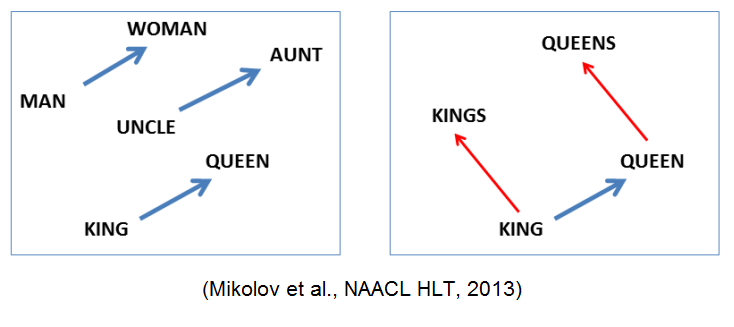
\includegraphics[width=10cm]{kingqueen.png}
	\caption{Semantic relationships between words as arrows in the vector space. \citep{WordVecLingReg}}
	\label{fig:w2vg}
\end{figure}

\begin{figure}[p]
	\centering
	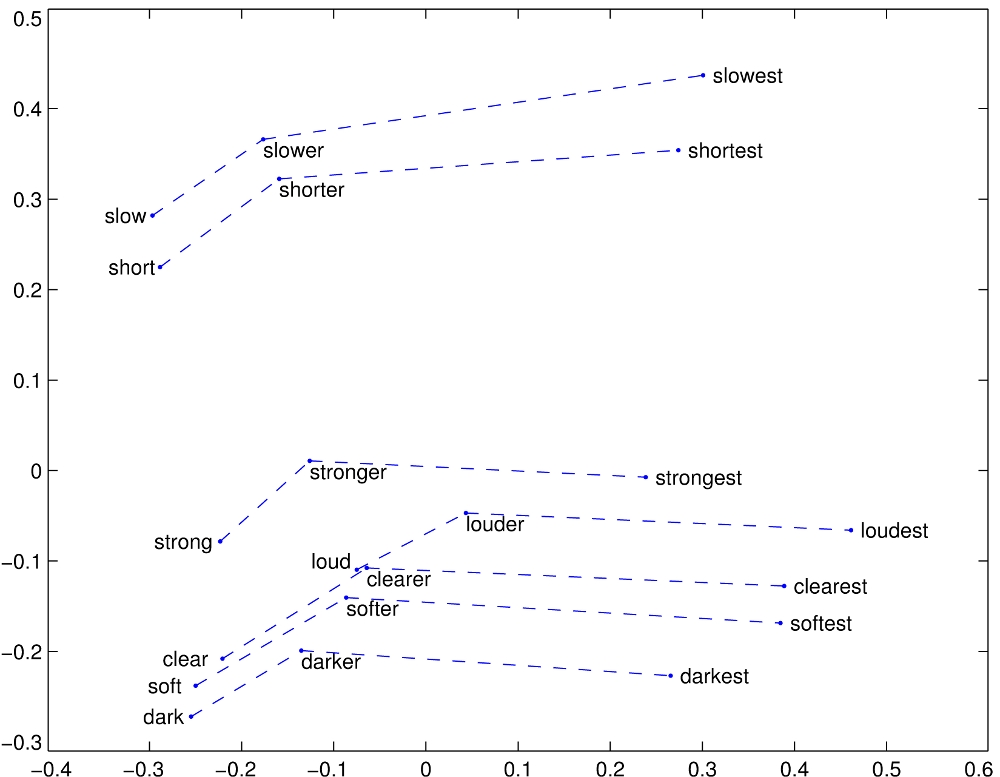
\includegraphics[width=10cm]{comparative_superlative.jpg}
	\caption{Semantic relationships between superlative adjectives as represented in the vector space.
		This is a 2D projection of the high-dimensional space that is designed to well preserve relative positions of the shown entities
		(so-called t-SNE 2D).
		\citep{Glove}}
	\label{fig:w2ver}
\end{figure}

\begin{figure}[p]
	\centering
	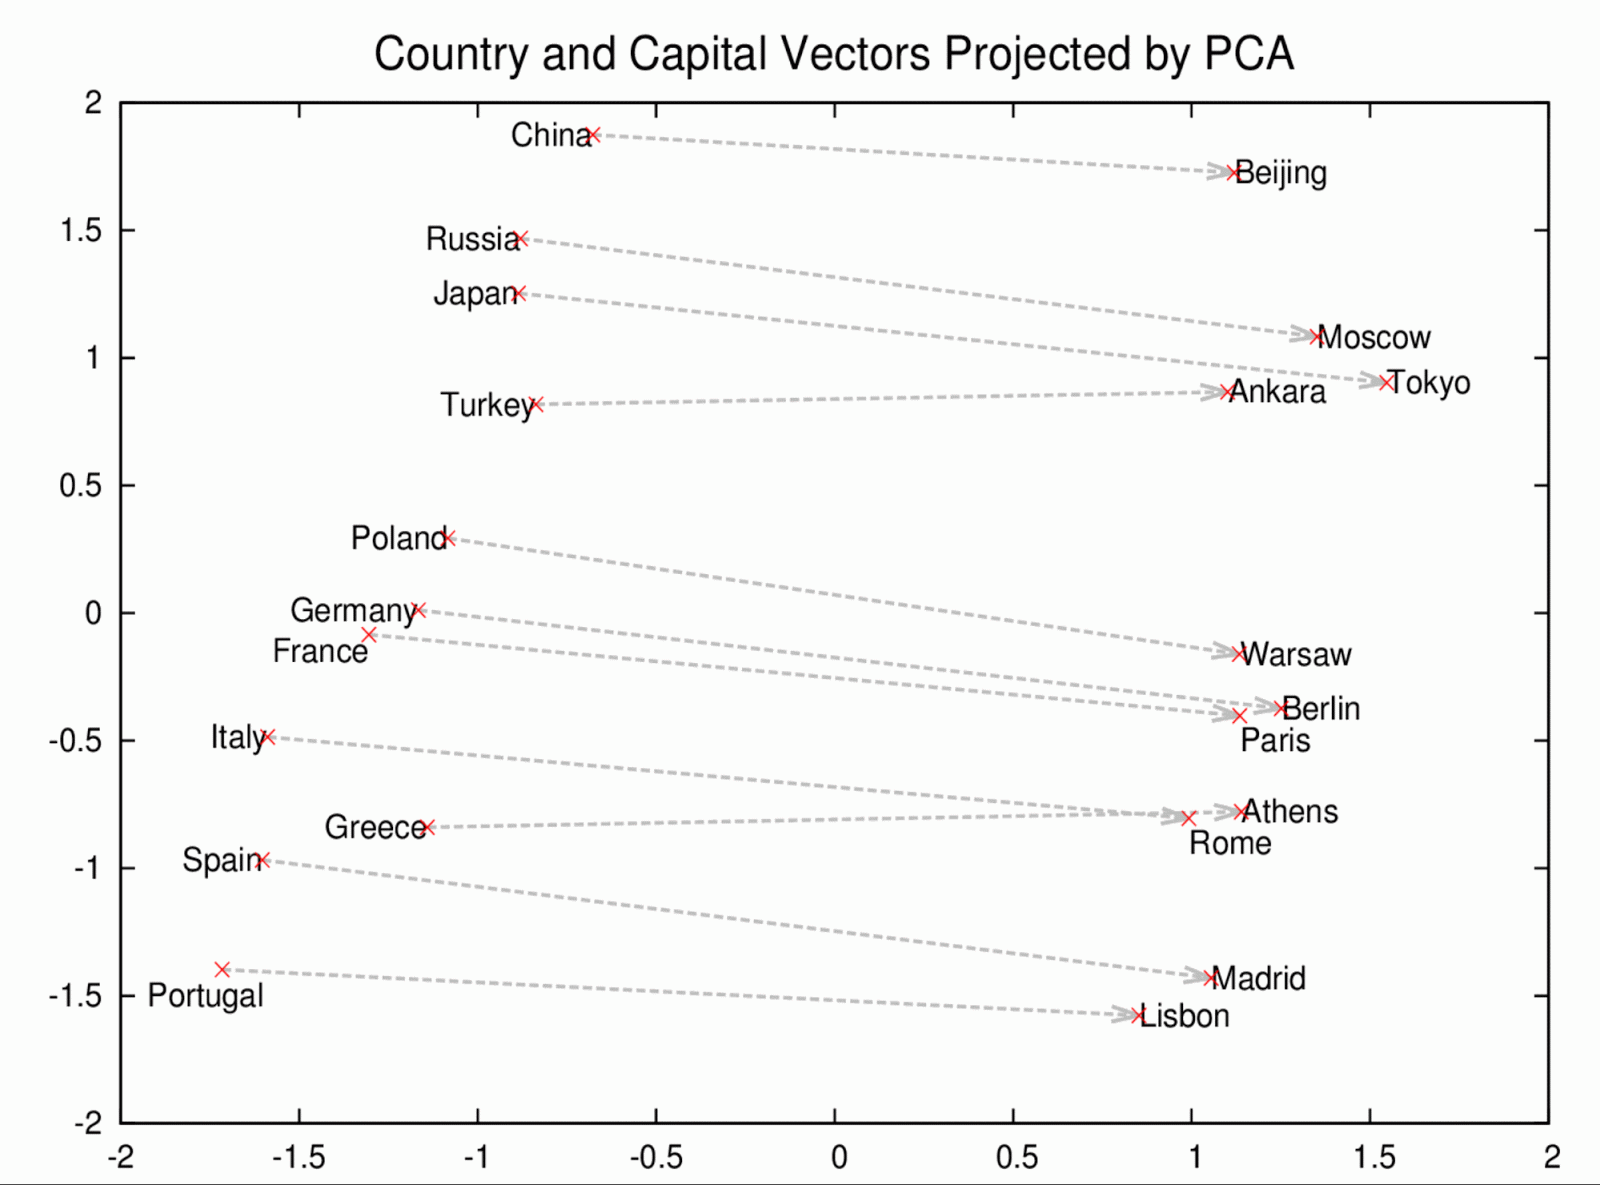
\includegraphics[width=11cm]{capitals.png}
	\caption{Mappings between countries and capitals, acquired entirely from the typical context of the respective words.
	This is again a 2D projection of the high-dimensional space, this time obtained by a PCA dimensionality reduction technique.
	\citep{DistReprComp}}
	\label{fig:w2vc}
\end{figure}

A lot of the current research focuses on the best ways to build up
vector representations of whole sentences and documents --- ranging
from simple averaging \citep{CNNSentClass,DefGen} (successful baselines)
to recurrent neural networks \citep{LISA,ShowAndTell}.
Many applications that rely on semantic understanding of word nuances
are popping up; this method became state-of-art for machine translation
\citep{LISA}, automatic image captioning \citep{ShowAndTell} and specific
types of question answering \citep{QANTA,DefGen,ReadAndComprehend}%
\footnote{The demo at \url{http://45.55.181.170/defgen/} is nice.}.
One open problem is efficient composition of vector embeddings for
common words with entities like numbers or proper names.
